\section{Experiments}\label{sec:experiments}
\lettrine[lines=3]{N}{}ext, we evaluate the performance of Titans and its variants in language modeling, commonsense reasoning, needle in haystack, DNA modeling, and time series forecasting tasks\footnote{In the first version of the work, we aim to provide insights/evidences about why the learning paradigms of Titans are effective. We are working on finalizing the results of larger models and will report them in the next version.}. In more details, in this section, we answer the following empirical questions: (1) How do Titans perform compared to baselines in downstream tasks? (\textcolor{c1}{see \S}\ref{sec:exp-lm}, \textcolor{c1}{\S}\ref{sec:exp-timeseries}, \textcolor{c1}{and \S}\ref{sec:exp-DNA}); (2) What is the actual context length of Titans? (\textcolor{c1}{see \S}\ref{sec:exp-hystack} \textcolor{c1}{and \S}\ref{sec:exp-babilong}); (3) How do Titans scale with respect to context length? (\textcolor{c1}{see \S}\ref{sec:exp-efficiency}); (4) How the depth of memory can affect both performance and efficiency? (\textcolor{c1}{see \S}\ref{sec:deep-memory-exp}); and (5) What is the contribution of each Titans' component in its performance? (\textcolor{c1}{see~\S}\ref{sec:exp-ablation}).

\subsection{Experimental Setup}\label{sec:exp-setup}
\head{Models}
In our experiments, we focus on the three variants of Titans, which we refer to as: Titans with (1) Memory as a Context (MAC), (2) Memory as a Gate (MAG), and (3) Memory as a Layer (MAL) as well as (4) neural memory module alone. The reason behind using our long-term memory as a separate module is based on our definition of learning. As discussed in \autoref{sec:intro}, we define learning a process for acquiring effective and useful memory. Accordingly, we expect our long-term memory to effectively learn from data, even without attention. For each of these models, we consider four scales with: (i) 170M, (ii) 340M,  (iii) 400M, and (iv) 760M parameters. While the first three are trained on 15B tokens sampled from FineWeb-Edu dataset~\citep{penedo2024the}, the last one is trained on 30B tokens from the same dataset. 




\begin{table*}[t!]
\centering
\caption{
Performance of Titans and recurrent- and Transformer-based baselines on language modeling and common-sense reasoning tasks. Hybrid models are marked with $^*$. The best results among {\colorbox{myblue}{simple}} and {\colorbox{mygreen}{hybrid}} models are highlighted. 
}\label{tab:lm_results}
\centering
\resizebox{0.9\linewidth}{!}{
\centering
\begin{tabular}{l|c c|c c c c c c c c c}
\toprule
\textbf{Model}  & \textbf{Wiki.}  &  \textbf{LMB.} &  \textbf{LMB.} & \textbf{PIQA} &    \textbf{Hella.} & \textbf{Wino.} & \textbf{ARC-e} &  \textbf{ARC-c} &  \textbf{SIQA}  & \textbf{BoolQ} &  \textbf{Avg.} \\
 & ppl $\downarrow$  &  ppl $\downarrow$  &  acc $\uparrow$  & acc $\uparrow$ &   acc\_n $\uparrow$  & acc $\uparrow$  & acc $\uparrow$ & acc\_n $\uparrow$ &  acc $\uparrow$  & acc $\uparrow$ &   $\uparrow$  \\
\midrule
\midrule
\multicolumn{12}{c}{340M params / 15B tokens} \\
\midrule
 Transformer++ & 31.52 & 41.08 &  30.76 & 62.98  &  34.76 & 50.53  & 45.21  & 24.05 & 36.81 & 58.24 & 42.92\\
 RetNet & 32.50 & 49.73 & 28.24 & 62.61 & 34.15 &  50.91 & 44.27 & 23.62 & 36.79 & 59.72 & 42.54\\
 GLA & 28.51 & 43.02 & 28.73 & 64.05 & 35.96 & 50.00 & 54.19 & 24.29 & 37.13 & 58.39 & 44.09\\
 Mamba & 30.83 & 40.21 & 29.94 & 63.79 & 35.88 & 49.82 & 49.24 & 24.56 &  35.41  & 60.07 & 43.59\\
 DeltaNet & 28.65 & 47.30 & 28.43 & 63.52 & 35.95 & 49.63 & 52.68 & 25.37 &  \cellcolor{myblue}\underline{37.96}  &  58.79  & 44.04 \\
 TTT & 27.44 & 34.19 & 30.06 & 63.97  & 35.71 & 50.08 & 53.01 & 26.11 & 37.32 & 59.83 & 44.51\\
 Gated DeltaNet & 27.01 & 30.94 &  34.11 & 63.08 & 38.12  &  51.60  &  55.28  &  26.77  & 34.89 & 59.54  & 45.42\\
\midrule
Titans (LMM) & \cellcolor{myblue}26.18 &  \cellcolor{myblue}29.97 &  \cellcolor{myblue}34.98  & \cellcolor{myblue}64.73  & \cellcolor{myblue}39.61  & \cellcolor{myblue}51.85  & \cellcolor{myblue}55.60  & \cellcolor{myblue}28.14 & 34.52 & \cellcolor{myblue}59.99 & \cellcolor{myblue} 46.17 \\
Titans (MAC)$^*$         & 25.43 & \cellcolor{mygreen}28.13  & 36.00 & \cellcolor{mygreen}65.32 & 40.35 & 51.21& \cellcolor{mygreen}58.17 & \cellcolor{mygreen}29.00 & 38.63 & \cellcolor{mygreen}60.18 & 47.36\\
Titans (MAG)$^*$         & 25.07 & 28.72 & \cellcolor{mygreen}36.71 & 64.88 & \cellcolor{mygreen}40.56 & \cellcolor{mygreen}52.49 & 57.72& 28.16 & \cellcolor{mygreen}39.75 & 60.01& \cellcolor{mygreen}47.54 \\
Titans (MAL)$^*$         & \cellcolor{mygreen}24.69 & 28.80 & 35.74  & 64.97 & 39.44 & 51.97 & 56.58  & 28.21 & 38.14 & 57.32 & 46.55\\
\midrule
\multicolumn{12}{c}{400M params / 15B tokens} \\
\midrule
 Transformer++ & 30.63 & 37.37 & 29.64 & 64.27 & 37.72 &	51.53 & 54.95	& 27.36 &  38.07  &  \cellcolor{myblue}\underline{61.59}  & 45.64 \\
 RetNet & 29.92 & 46.83 & 29.16 & 65.23 & 36.97 &	51.85 & 56.01	& 27.55 &  37.30  & 59.66  & 45.47 \\
 HGRN2 & 32.33 & 47.14 & 26.12 & 64.52 & 35.45 &	52.24 & 55.97	& 25.51 &  37.35  & 59.02  & 44.52 \\
GLA & 27.96 & 36.66 & 27.86 &  \cellcolor{myblue}\underline{65.94} & 37.41 &	49.56 & 56.01	& 26.36 &   \cellcolor{myblue}\underline{38.94}  & 59.84  & 45.24 \\
 Mamba & 29.22 & 39.88 & 29.82 & 65.72 & 37.93 &	50.11 & 58.37	& 26.70 &  37.76  & 61.13  & 45.94 \\
Mamba2 & 26.34 & 33.19 & 32.03 & 65.77 & 39.73 &	{52.48} & 59.00	& 27.64 &  37.92  & 60.72  & 46.91 \\
 DeltaNet & 27.69 & 44.04 & 29.96 & 64.52 & 37.03 &	50.82 & 56.77	& 27.13 &  38.22  & 60.09  & 45.57 \\
 TTT & 26.11 & 31.52 & 33.25 & 65.70 & 39.11 & 51.68& 58.04& 28.99 & 38.26 & 59.87 & 46.86\\
Gated DeltaNet & 25.47 & 29.24 & 34.40 &  \cellcolor{myblue}\underline{65.94} & 40.46 &	51.46 & {59.80}	& {28.58} &  37.43  & 60.03  & 47.26 \\
 Samba$^*$ & 25.32 & 29.47 & 36.86 & 66.09& 39.24 & 51.45 & 60.12 & 27.20  & 38.68  &  58.22 & 47.23\\
Gated DeltaNet-H2$^*$  & {24.19} & {28.09} & {36.77} & {66.43} & {40.79} &	{52.17} & 59.55	& {29.09} &  {39.04}  & 58.56  & {47.69} \\
\midrule
Titans (LMM) & \cellcolor{myblue}25.03 & \cellcolor{myblue} 28.99  & \cellcolor{myblue}35.21 & 65.85 & \cellcolor{myblue}40.91 & \cellcolor{myblue}52.19 & \cellcolor{myblue} 59.97 & \cellcolor{myblue}29.20 & 38.74 & 60.85 &  \cellcolor{myblue}47.83  \\
Titans (MAC)$^*$         & 25.61 & \cellcolor{mygreen}27.73  &     36.92 & 66.39 & \cellcolor{mygreen}41.18 & 52.80 & \cellcolor{mygreen}60.24 & 29.69 & \cellcolor{mygreen}40.07  & \cellcolor{mygreen}61.93 & \cellcolor{mygreen}48.65 \\
Titans (MAG)$^*$         & \cellcolor{mygreen}23.59 & 27.81  & \cellcolor{mygreen}37.24 & \cellcolor{mygreen}66.80 & 40.92 &  \cellcolor{mygreen}53.21 & 60.01 & 29.45 & 39.91 & 61.28 & 48.60 \\
Titans (MAL)$^*$         & 23.93 & 27.89  & 36.84 & 66.29 & 40.74 & 52.26 &  59.85 & \cellcolor{mygreen}29.71 & 38.92 & 58.40 & 47.87 \\
\midrule
\multicolumn{12}{c}{760M params / 30B tokens} \\
\midrule
 Transformer++ & 25.21 & 27.64 & 35.78 & 66.92 & 42.19 &	51.95 & 60.38	& 32.46 &  39.51  & 60.37  & 48.69 \\
 RetNet & 26.08 & 24.45 & 34.51 & 67.19 & 41.63 &	52.09 & 63.17	& 32.78 &  38.36  & 57.92  &  48.46\\
 Mamba & 28.12 & 23.96 & 32.80 & 66.04 & 39.15 &	\cellcolor{myblue}\underline{52.38} & 61.49	& 30.34 &  37.96  & 57.62  & 47.22 \\
 Mamba2 & 22.94 & 28.37 & 33.54 & 67.90 & 42.71 &	49.77 & {63.48}	& 31.09 &  40.06  & 58.15  & 48.34 \\
 DeltaNet & 24.37 & 24.60 & 37.06 & 66.93 & 41.98 &	50.65 & 64.87	& 31.39 &  39.88  & 59.02  & 48.97 \\
 TTT & 24.17 & 23.51 & 34.74 & 67.25 & 43.92 & 50.99 & 64.53 & 33.81 & \cellcolor{myblue}\underline{40.16} & 59.58 & 47.32 \\
 Gated DeltaNet & {21.18} & {22.09} & {35.54} & {68.01} & {44.95} & {50.73} & \cellcolor{myblue}\underline{66.87}	& {33.09} &  {39.21}  & 59.14  & 49.69 \\
 Samba$^{*}$ & 20.63 & 22.71 & 39.72 & 69.19 & 47.35 &	52.01 & 66.92	& 33.20 &  38.98  & 61.24  & 51.08 \\
  Gated DeltaNet-H2$^*$ & {19.88} & 20.83 & {39.18} & 68.95 & {48.22} &	{52.57} & 67.01	& {35.49} &  {39.39}  & 61.11  & 51.49 \\
  \midrule
Titans (LMM) & \cellcolor{myblue}20.04 & \cellcolor{myblue}21.96 &  \cellcolor{myblue}37.40 & \cellcolor{myblue}69.28  & \cellcolor{myblue}48.46 & 52.27 & 66.31 & \cellcolor{myblue}35.84 & 40.13 & \cellcolor{myblue}62.76 & \cellcolor{myblue}51.56\\
Titans (MAC) & 19.93 & 20.12 &  39.62 & \cellcolor{mygreen}70.46  & \cellcolor{mygreen}49.01 & \cellcolor{mygreen}53.18 & 67.86 & 36.01 & \cellcolor{mygreen}41.87 & \cellcolor{mygreen}62.05 & \cellcolor{mygreen}52.51\\
Titans (MAG) & \cellcolor{mygreen}18.61 & \cellcolor{mygreen}19.86 &  \cellcolor{mygreen}40.98 & 70.25  & 48.94 & 52.89 & \cellcolor{mygreen}68.23 & \cellcolor{mygreen}36.19 & 40.38 & 62.11 & 52.50\\
Titans (MAL) & 19.07 & 20.33 &  40.05 & 69.99  & 48.82 & 53.02& 67.54 & 35.65 & 30.98 & 61.72 & 50.97\\
\bottomrule
\end{tabular}
}
\end{table*}

\head{Baselines}
We compare our models with the state-of-the-art linear recurrent models, Transformers, and hybrid models (recurrent + attention). More specifically in language tasks, we compare with Transformer++~\citep{touvron2023llama}, RetNet~\citep{sun2023retentive}, Gated Linear Attention (GLA)~\citep{yang2024gatedattn}, Mamba~\citep{gu2024mamba}, Mamba2~\citep{dao2024transformers}, DeltaNet~\citep{yang2024parallelizing}, TTT~\citep{sun2024learning}, and Gated DeltaNet~\citep{yang2024gated}. In needle in haystack tasks, we also compare with GPT4~\citep{achiam2023gpt}, Llama3 with RAG~\citep{touvron2023llama}, RecurrentGemma2-9B~\citep{botev2024recurrentgemma}, and Mistral~\citep{jiang2023mistral} models, all of which are provided in the benchmark~\citep{kuratov2024babilong}. In time series tasks, we compare with Mamba-based~\citep{behrouz2024mambamixer}, Transformer-based~\citep{nie2022time, liu2023itransformer, zhang2023crossformer}, and linear models~\citep{das2023longterm, wu2023timesnet, zeng2023transformers, li2023revisiting}. 

\head{Training}
In the training, we follow the training procedure of \citet{yang2024gated}, and use LLama 2 tokenizer with a vocabulary size of 32K and use training length of 4K tokens. We employ AdamW optimizer with learning rate of $4e$-$4$ with cosine annealing schedule with batch size of 0.5M tokens, and weight decay of $0.1$.   


\subsection{Language Modeling}\label{sec:exp-lm}
We first focus on the perplexity in language modeling and also commonsense reasoning tasks. The results for Titans' variants and also baselines with three different sizes of 340M, 400M, and 760M are reported in \autoref{tab:lm_results}. Among non-hybrid models, including Transformer++, our neural memory module achieves the best performance in both perplexity and accuracy measures. Comparing our neural memory module and TTT, which is also a gradient-based recurrent model can show us the importance of our weight decay as well as the momentum. As discussed earlier, the weight decay can be interpreted as a gating mechanism to forget the past data, when it is needed. Also, momentum can help us better manage the memory by providing additional memory for the surprise metric. While some baselines also take advantage of gating mechanism, e.g., Mamba, Mamba2, and Gated DeltaNet, the superior performance of our neural memory module shows the importance of both our surprise mechanism and having deep and non-linear memory. We further discuss the later in \autoref{sec:deep-memory-exp}. 

Comparing the hybrid models, we found that all three variants of Titans (MAC, MAG, and MAL) outperform both Samba (Mamba + attention) and Gated DeltaNet-H2 (Gated DeltaNet + atttention). We attribute the superior performance of Titans (MAL) to the power of neural memory module as the architecture design and used attention are all the same. Comparing Titans (MAG) and (MAC), we find that while their performance are close, MAC performs better when dealing with longer dependencies in the data. Interestingly, both MAG and MAC outperform MAL variant, which due to using the same modules, we attribute this to the architecture design of these models. This finding is particularly important as the current hybrid models (except Hymba~\citep{dong2024hymba}) in the literature are using MAL-style combination of recurrent models and attention. 



\begin{table*}
    \centering
    \caption{Performance of Titans and baselines on S-NIAH task from RULER benchmark. The best results among {\colorbox{myblue}{simple}} and {\colorbox{mygreen}{hybrid}} models are highlighted.}
    \label{tab:hystack}
    \resizebox{0.7\linewidth}{!}{
    \begin{tabular}{l c c c c c c c c c c c c}
    \toprule
    \multirow{2}{*}{Model} & \multicolumn{4}{c}{\textbf{S-NIAH-PK}} & \multicolumn{4}{c}{\textbf{S-NIAH-N}} & \multicolumn{4}{c}{\textbf{S-NIAH-W}} \\
    \cmidrule(lr){2-5} \cmidrule(lr){6-9} \cmidrule(lr){10-13}
    &  2K & 4K & 8K & 16K &  2K & 4K & 8K & 16K &  2K & 4K & 8K & 16K \\
    \midrule
    \midrule
       TTT  & 98.4 & \cellcolor{myblue}98.8 & 98.0 & 88.4 & 60.2 & 36.6 &  10.2 & 4.4 & 78.8 & 28.0 & 4.4 & 0.0 \\
       Mamba2 & 98.6 & 61.4 & 31.0 & 5.4 & 98.4 & 55.8 & 14.2 & 0.0 & 42.2 & 4.2 & 0.0 & 0.0\\
       DeltaNet & 96.8 & \cellcolor{myblue}98.8 & \cellcolor{myblue}98.6 & 71.4 & 47.2 & 15.4 & 12.8 & 5.4 & 46.2 & 20.0 & 1.6 & 0.0\\
       \midrule
       Titans (LMM) & \cellcolor{myblue}99.8 & 98.4 & 98.2 & \cellcolor{myblue}96.2 & \cellcolor{myblue}100.0 & \cellcolor{myblue}99.8 & \cellcolor{myblue}93.4 & \cellcolor{myblue}80.2 & \cellcolor{myblue}90.4 & \cellcolor{myblue}89.4 & \cellcolor{myblue}85.8 & \cellcolor{myblue}80.6 \\
       Titans (MAC)  & 99.2 & \cellcolor{mygreen}98.8 & \cellcolor{mygreen}99.0 & \cellcolor{mygreen}98.4 & 99.6 & 98.2 & \cellcolor{mygreen}97.6 & 97.4  & \cellcolor{mygreen}98.2 & \cellcolor{mygreen}98.2 & \cellcolor{mygreen}95.6 & \cellcolor{mygreen}95.2 \\
       Titans (MAG) & \cellcolor{mygreen}99.4 & 98.0 & 97.4 & 97.4 & 99.2 & \cellcolor{mygreen}98.8 &  97.2 & \cellcolor{mygreen}98.6 &  98.0 & 98.0  & 90.2  &  88.2  \\
       Titans (MAL) & 98.8 & 98.6 & 98.8 & 97.8 & \cellcolor{mygreen}99.8  & 98.1 & 96.8  & 96.4 & 98.0 & 97.4 & 92.0 & 90.4\\
    \toprule
    \end{tabular}
    }
\end{table*}

\subsection{Needle in a Haystack}\label{sec:exp-hystack}
Scaling a model to longer context window is not always equivalent to being effective for very long sequences~\citep{hsieh2024ruler}. The needle-in-a-haystack (NIAH) task is designed to measure the actual effective context length of models. In this task, we evaluate the model on retrieving a piece of information (i.e., the ``needle'') from long distractor texts (i.e., the ``haystack''). In this part, we use Single NIAH (S-NIAH) task from RULER benchmark~\citep{hsieh2024ruler} and evaluate Titans and baselines on sequences with length 2K, 4K, 8K, and 16K. The results are reported in \autoref{tab:hystack}. Neural Memory module achieves the best results compare to baselines in all three tasks. We attribute this superior performance to three key differences of Titans with existing sequence models: (1) Compared to TTT, our Neural Memory can better handle the memory capacity by using momentum and also the forgetting mechanism (i.e., weight decay). Therefore, with increasing the sequence length, the performance of Neural Memory does not drop and show a consistent trend; (2) Compared to Mamba2, which has the gating (forgetting) mechanism, Titans have deep non-linear memory, resulting in better memory management. Also, contrary to our neural memory and DeltaNet, Mamba2 is not capable of removing a memory and so we can see a significant drop in performance when increasing the sequence length; (3) Compared to DeltaNet, although it is capable of removing memory using delta rule, it cannot erase the memory, lacking forgetting mechanism. Finally, As expected we can see on par or better results when using Titans variants, where the best results correspond to MAC.  




\begin{figure*}[t!]
    \centering
    \begin{subfigure}{0.33\linewidth}
        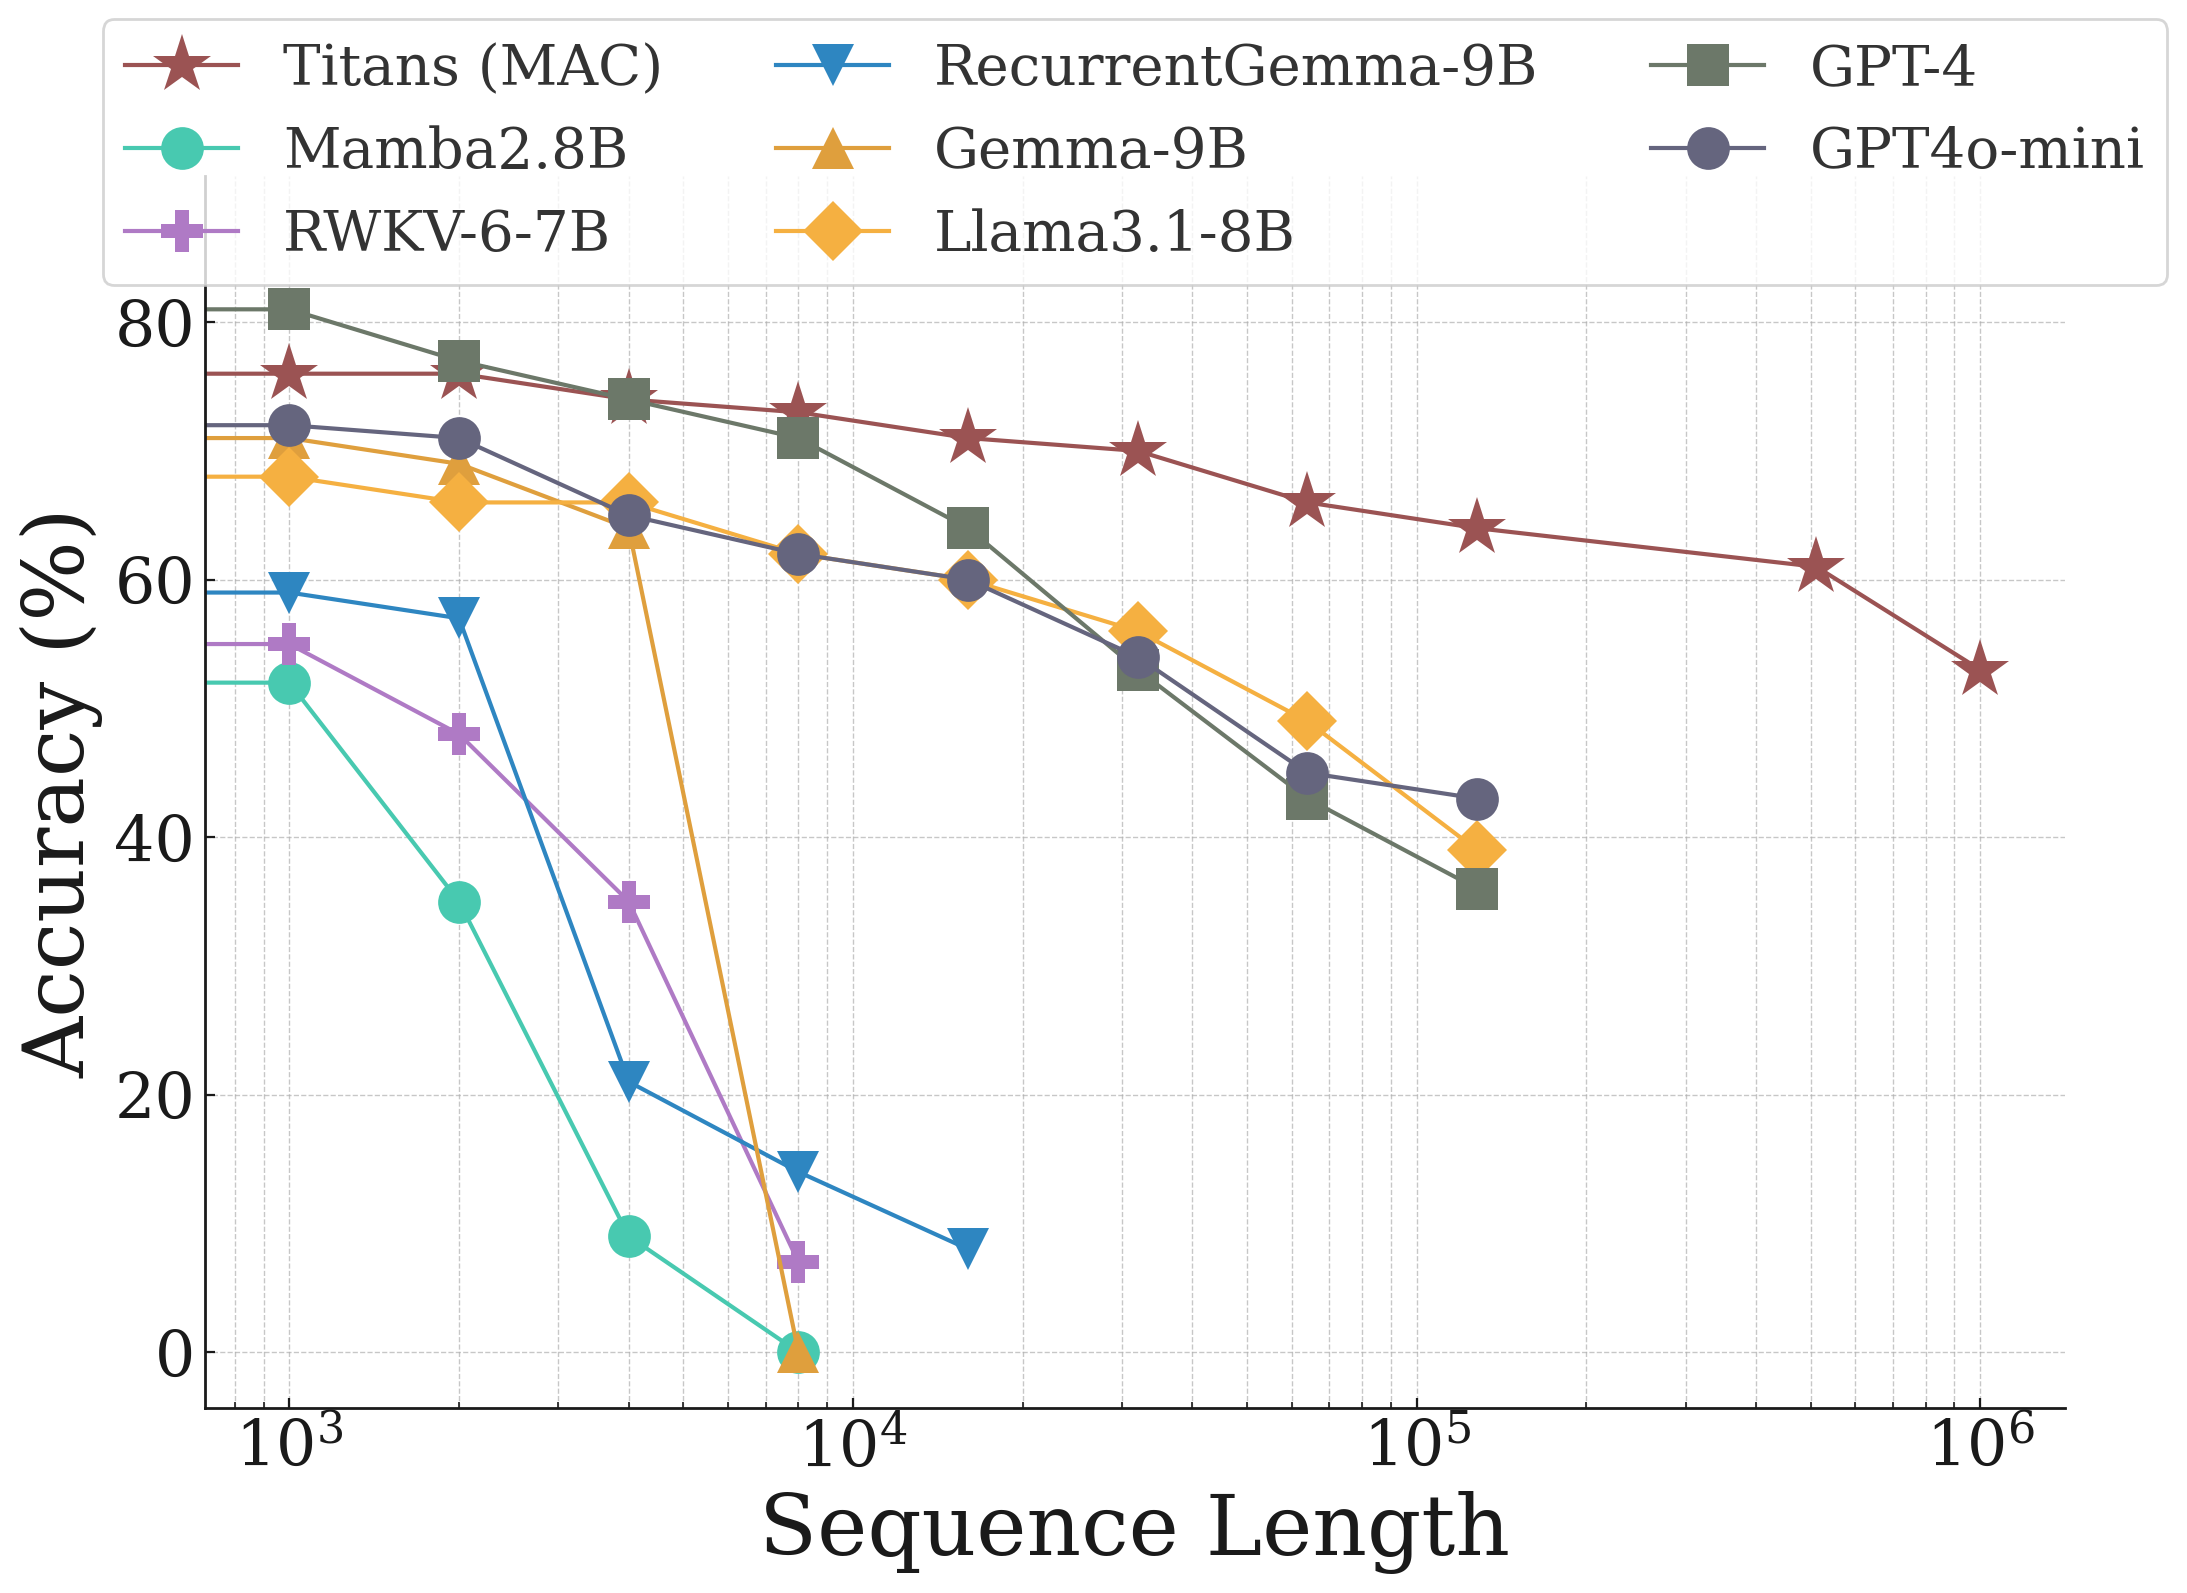
\includegraphics[width=\linewidth]{Figures/BABILong-few-shot.png}
    \caption{Few-shot Setup}
    \label{fig:babilong-zero-shot}
    \end{subfigure}~
    \centering~\hspace{4ex}
    \begin{subfigure}{0.33\linewidth}
        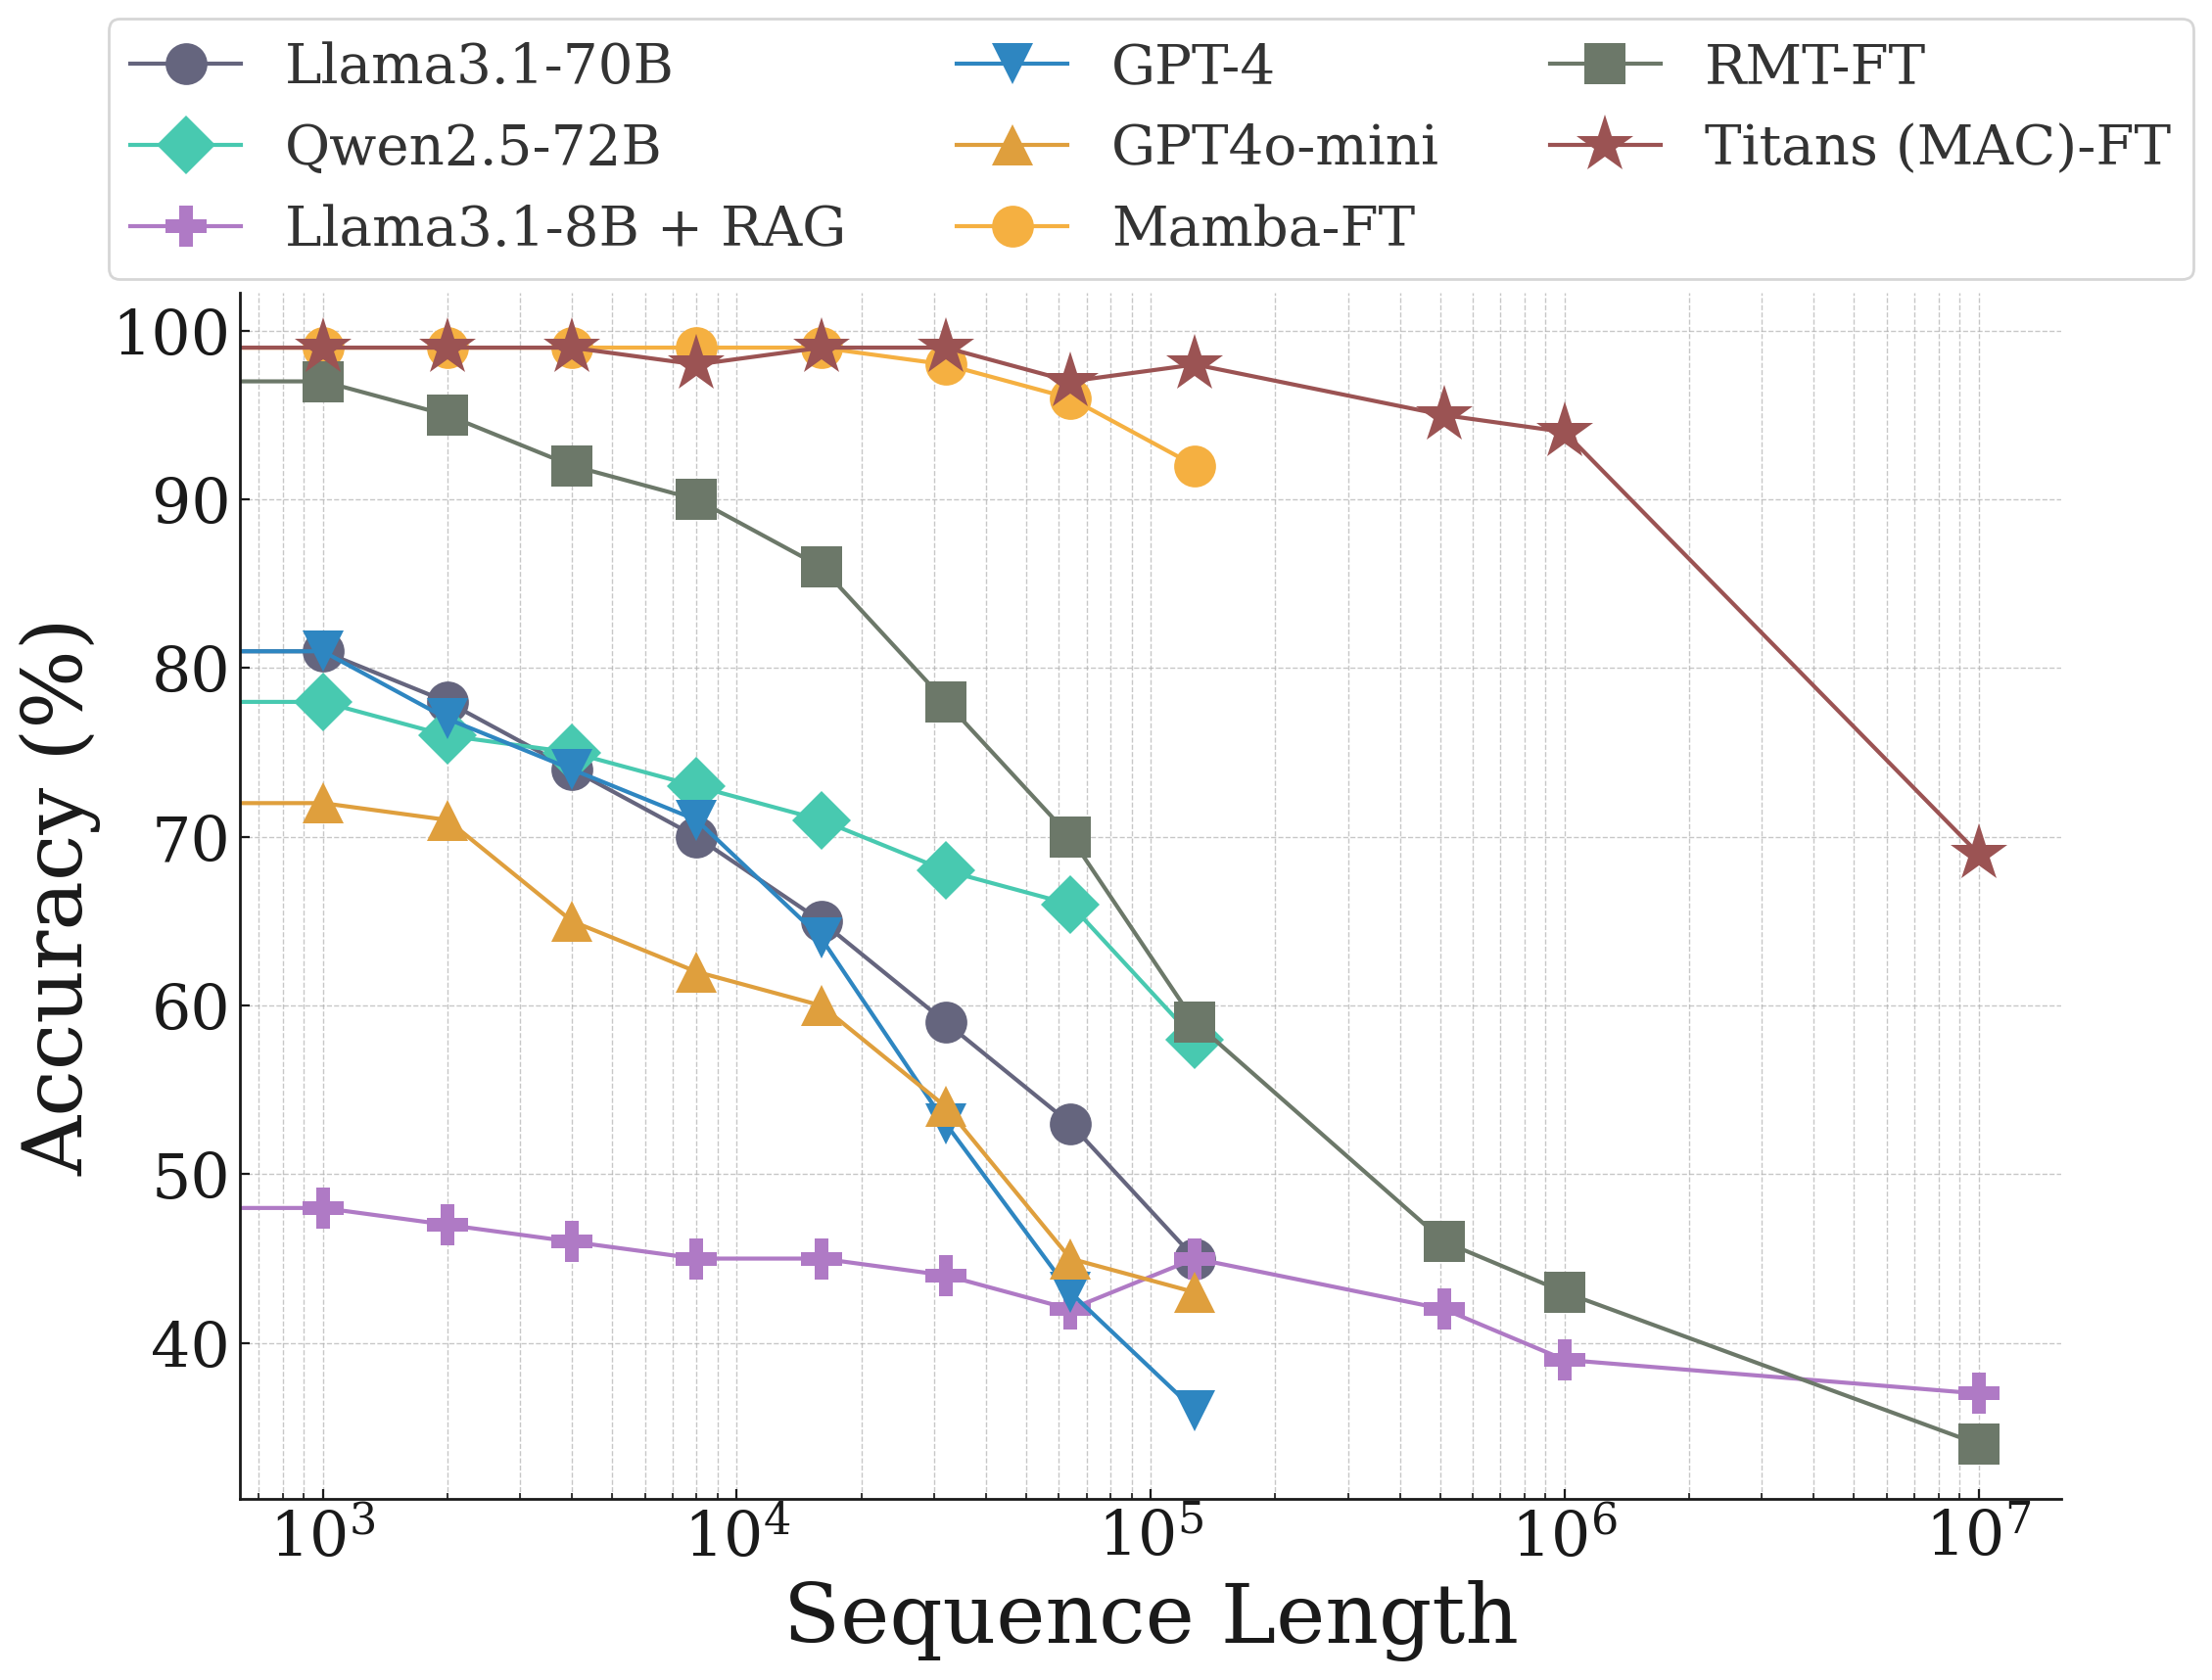
\includegraphics[width=\linewidth]{Figures/BABILong-FT.png}
    \caption{Fine-Tuning Setup}
    \label{fig:babilong-fine-tune}
    \end{subfigure}
    \caption{Performance of Titans and baselines on BABILong benchmark. Titans (MAC) outperforms all baselines, including extremely large models, e.g., GPT4.}
    \vspace{-2ex}
\end{figure*}



\subsection{BABILong Benchmark}\label{sec:exp-babilong}
In the previous section we discussed the results on a simple NIAH tasks where a single needle needs to be retrieved. Although Titans showed better performance compared to baselines, their true advantage over very long sequences is still hidden. To this end, in this section, we use a harder task from BABILong benchmark~\citep{kuratov2024babilong}, in which the model needs to reason across facts distributed in extremely long documents. We follow the original experimental setup and training process in the benchmark. There are two settings: (1) Few-shot setting, in which we use large pre-trained models, and (2) fine-tuning setting, where we fine-tune the MAC variant of Titans to compare it with other fine-tuned baselines. The results for few-shot setting are reported in \autoref{fig:babilong-zero-shot}. In this setup, we can see Titans outperform all baselines–i.e., Mamba2.8B~\citep{gu2024mamba}, RWKV-6-7B~\citep{peng2024eagle}, RecurrentGemma-9B~\citep{botev2024recurrentgemma}, Gemma-9B~\citep{team2024gemma}, Llama3.1-8B~\citep{touvron2023llama}, GPT-4, and GPT4o-mini~\citep{achiam2023gpt}. These results are achieved while Titans (MAC) is having much less number of parameters than baselines. 


In the fine-tuning setup, we compare the small fine-tuned version of Titans (MAC) with: (i) the fine-tuned version of small models (almost the same number of parameters as Titans) such as Mamba~\citep{gu2024mamba}, RMT~\citep{bulatov2022recurrent}, (ii) large models with Retrieval-Augmented Generation (RAG)~\citep{lewis2020retrieval} such as Llama3.1-8B~\citep{touvron2023llama}, and (iii) extremely large models such as GPT-4~\citep{achiam2023gpt}, GPT4o-mini, Qwen2.5-72B~\citep{yang2024qwen2}, and Llama3.1-70B~\citep{touvron2023llama}. Baseline results are reported by \citep{kuratov2024babilong}. The results of Titans and baselines are reported in \autoref{fig:babilong-fine-tune}. Titans outperform all models even extremely large models like GPT4. Also, compared to Transformer-based with memory models like RMT, Titans show better performance mainly due to their powerful memory. That is, RMT compress the historical data into 16 size vector-valued memory, while Titans with in-context online memory learner are capable of encoding the past into the parameters of the model. Interestingly, even augmenting Llama3.1-8B model with RAG performs worse than Titans with about $\times$70 less parameters.       










\begin{figure*}[t!]
    \centering
    \begin{subfigure}{0.333\linewidth}
        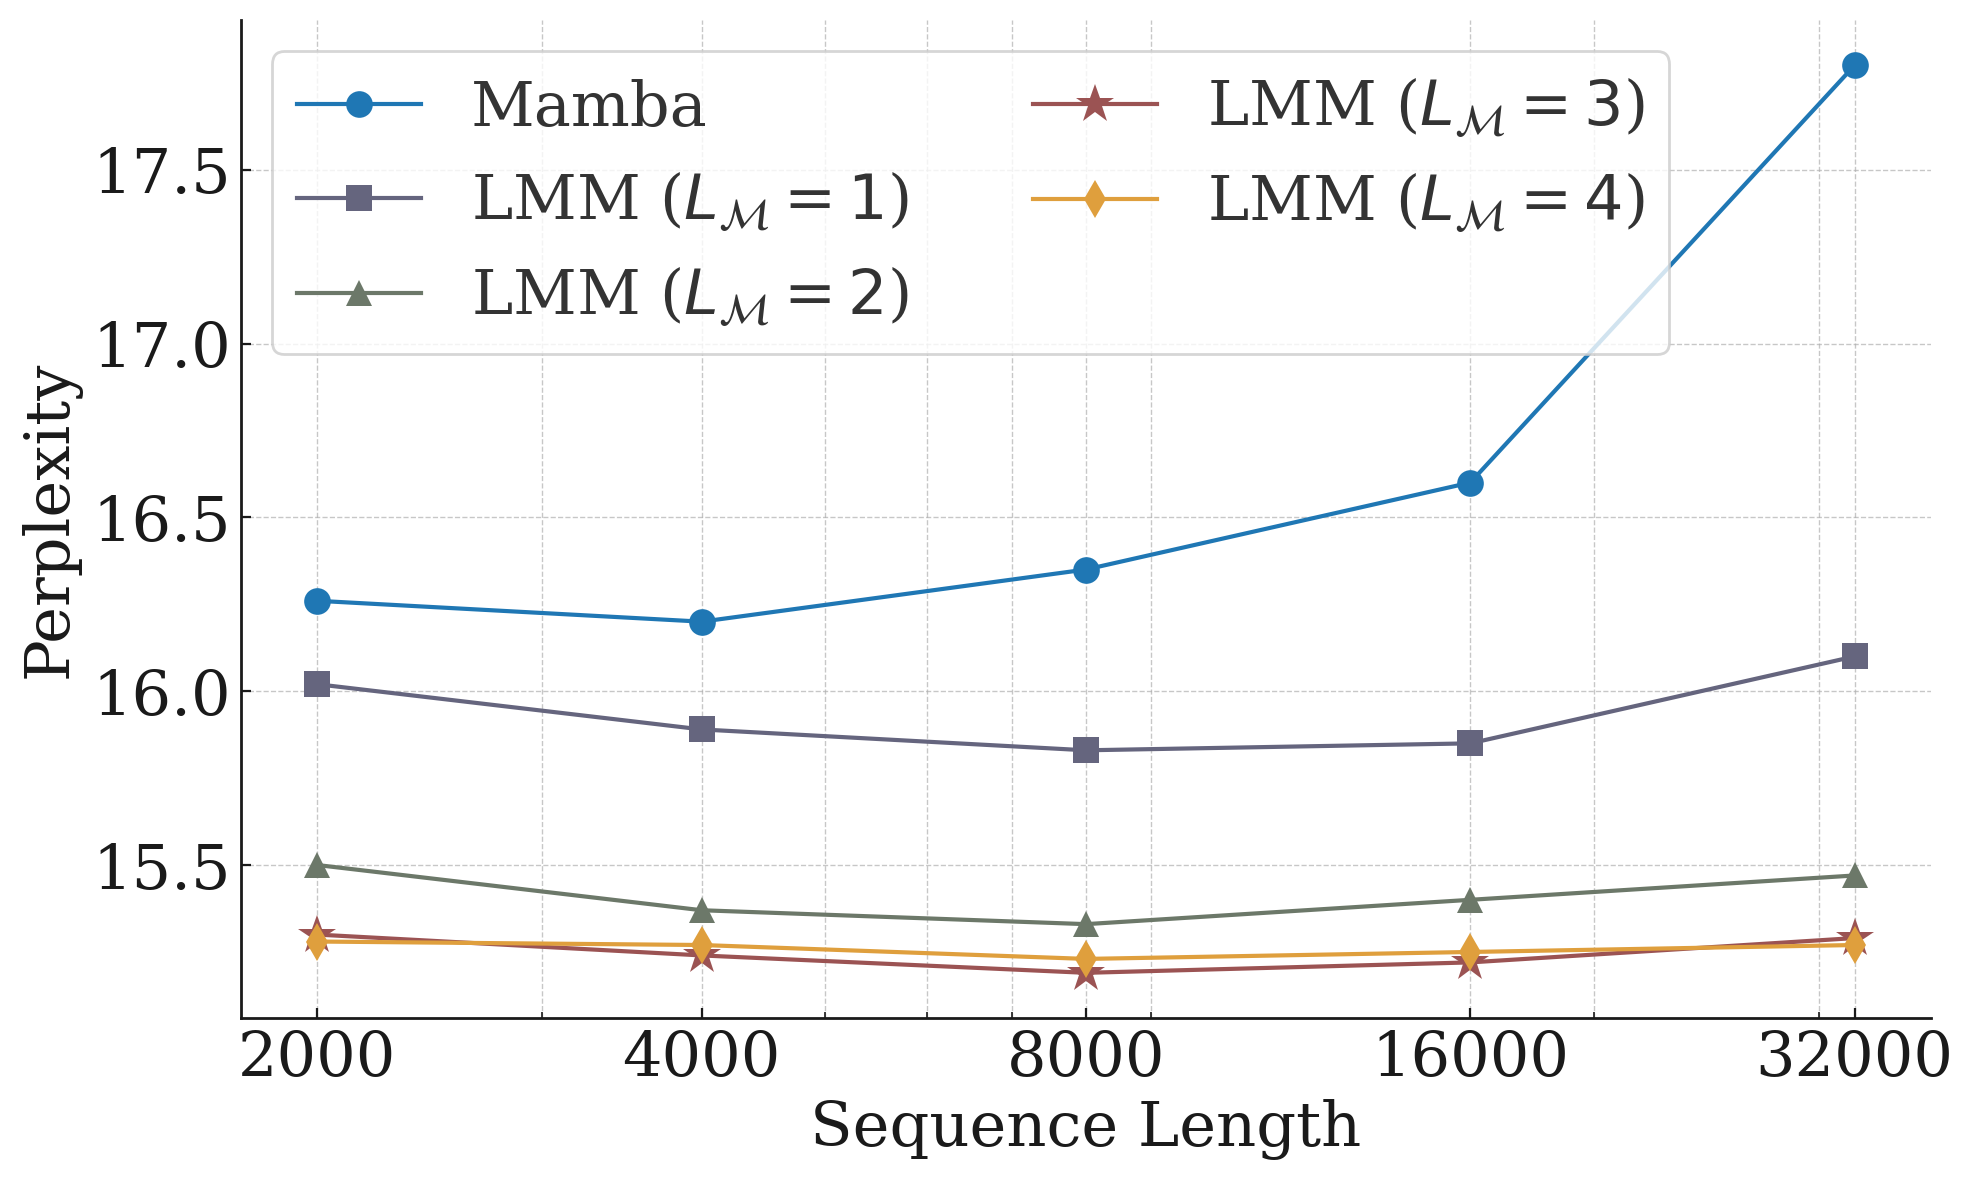
\includegraphics[width=\linewidth]{Figures/deep-memory-1.png}
    \caption{170M Parameters}
    \end{subfigure}~
    \centering
    \begin{subfigure}{0.333\linewidth}
        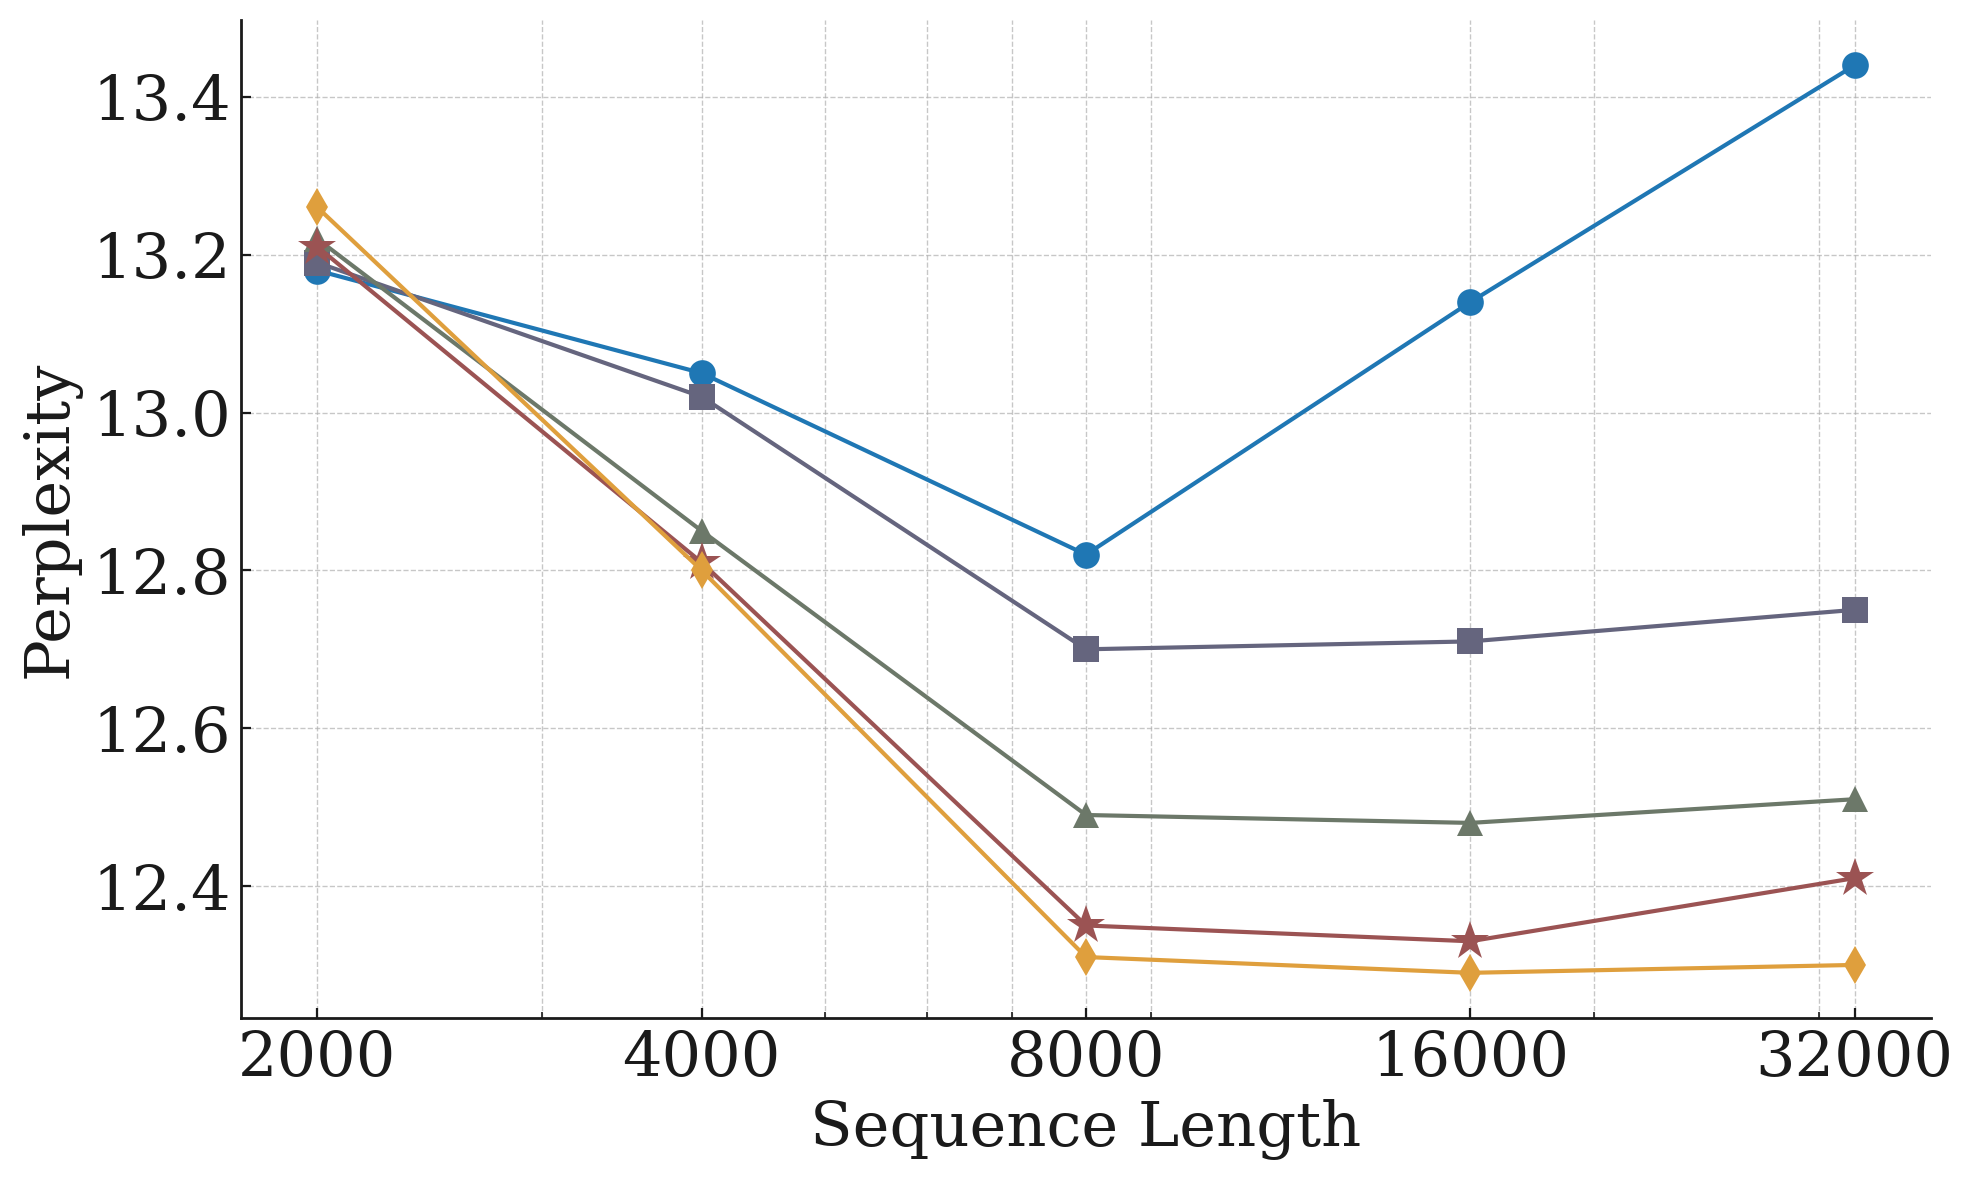
\includegraphics[width=\linewidth]{Figures/deep-memory-2.png}
    \caption{360M Parameters}
    \end{subfigure}~
    \centering
    \begin{subfigure}{0.333\linewidth}
        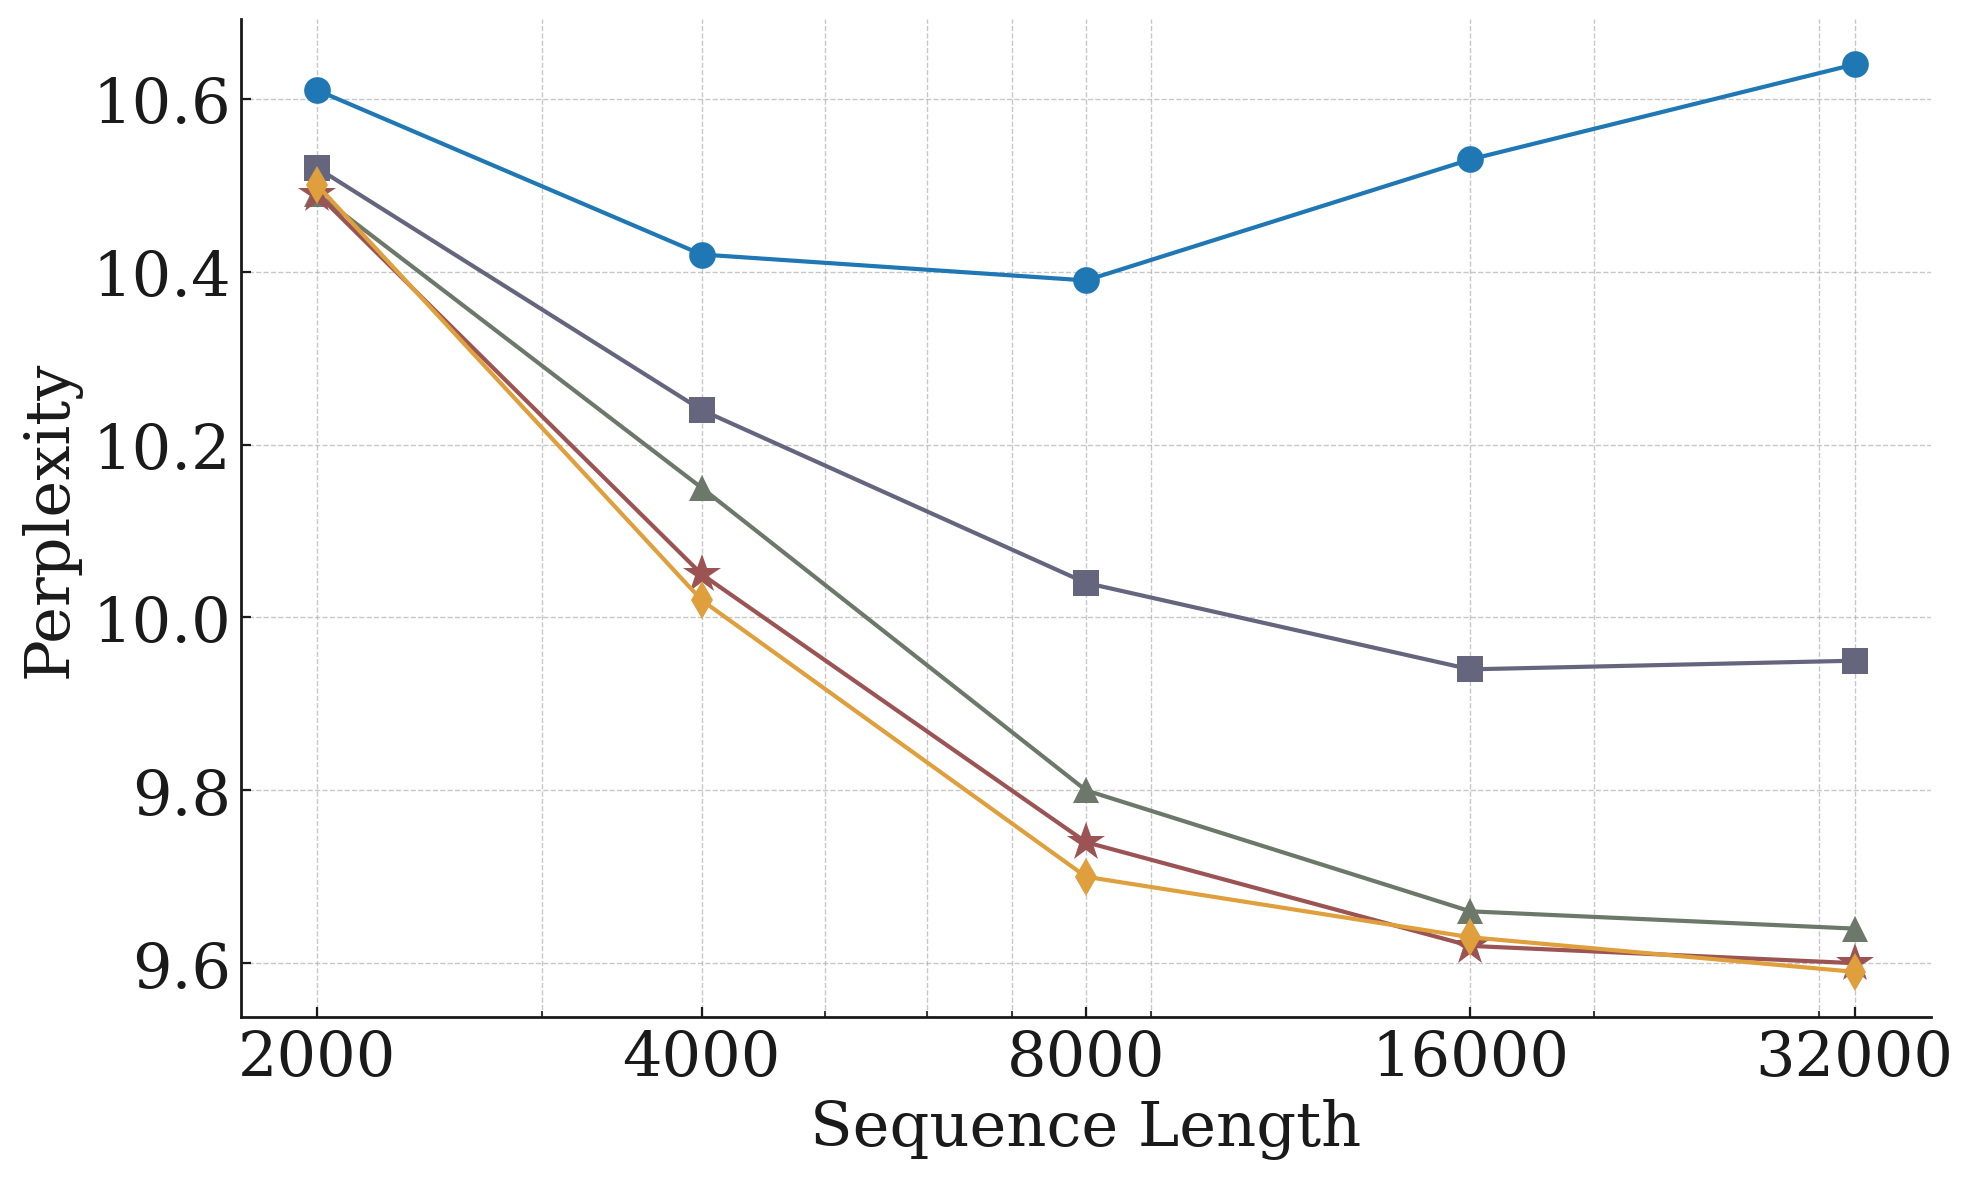
\includegraphics[width=\linewidth]{Figures/deep-memory-3.png}
    \caption{760M Parameters}
    \end{subfigure}
    \caption{The effect of memory depth on the perplexity. Deeper long-term memory results in better scaling in longer sequences.}
    \label{fig:effect-deep-memory}
\end{figure*}


\subsection{The Effect of Deep Memory}\label{sec:deep-memory-exp}
In this section, we evaluate the effect of deep memory in both wall-clock training time and model performance\footnote{Note that, in this experiment, we only focus on the neural memory module to evaluate the effect of memory depth in the memorization process. Combining neural memory with attention as we do in Titans variants, can additionally enhance the performance of the model over long sequences.}. To this end, we focus on different variants of our neural memory module, where $L_{\M} = 1, 2, 3, 4$. We also use Mamba as a baseline for the model performance. For a fair comparison, we use the same training process for all models and train them on a subset of the Pile dataset~\citep{gao2020pile}. 

We report the perplexity of our models and baselines as the function of the sequence length in \autoref{fig:effect-deep-memory}. Interestingly, with the increase of memory depth, $L_{\M}$, the model can achieve better perplexity over all sequence length. Also, deeper memory modules are more robust to the sequence length when the model has less number of parameters. With the increase of the number of parameters, all models show better performance on longer sequences.  


\begin{wrapfigure}{r}{0.33\linewidth}
    \centering
    \vspace{-4ex}
        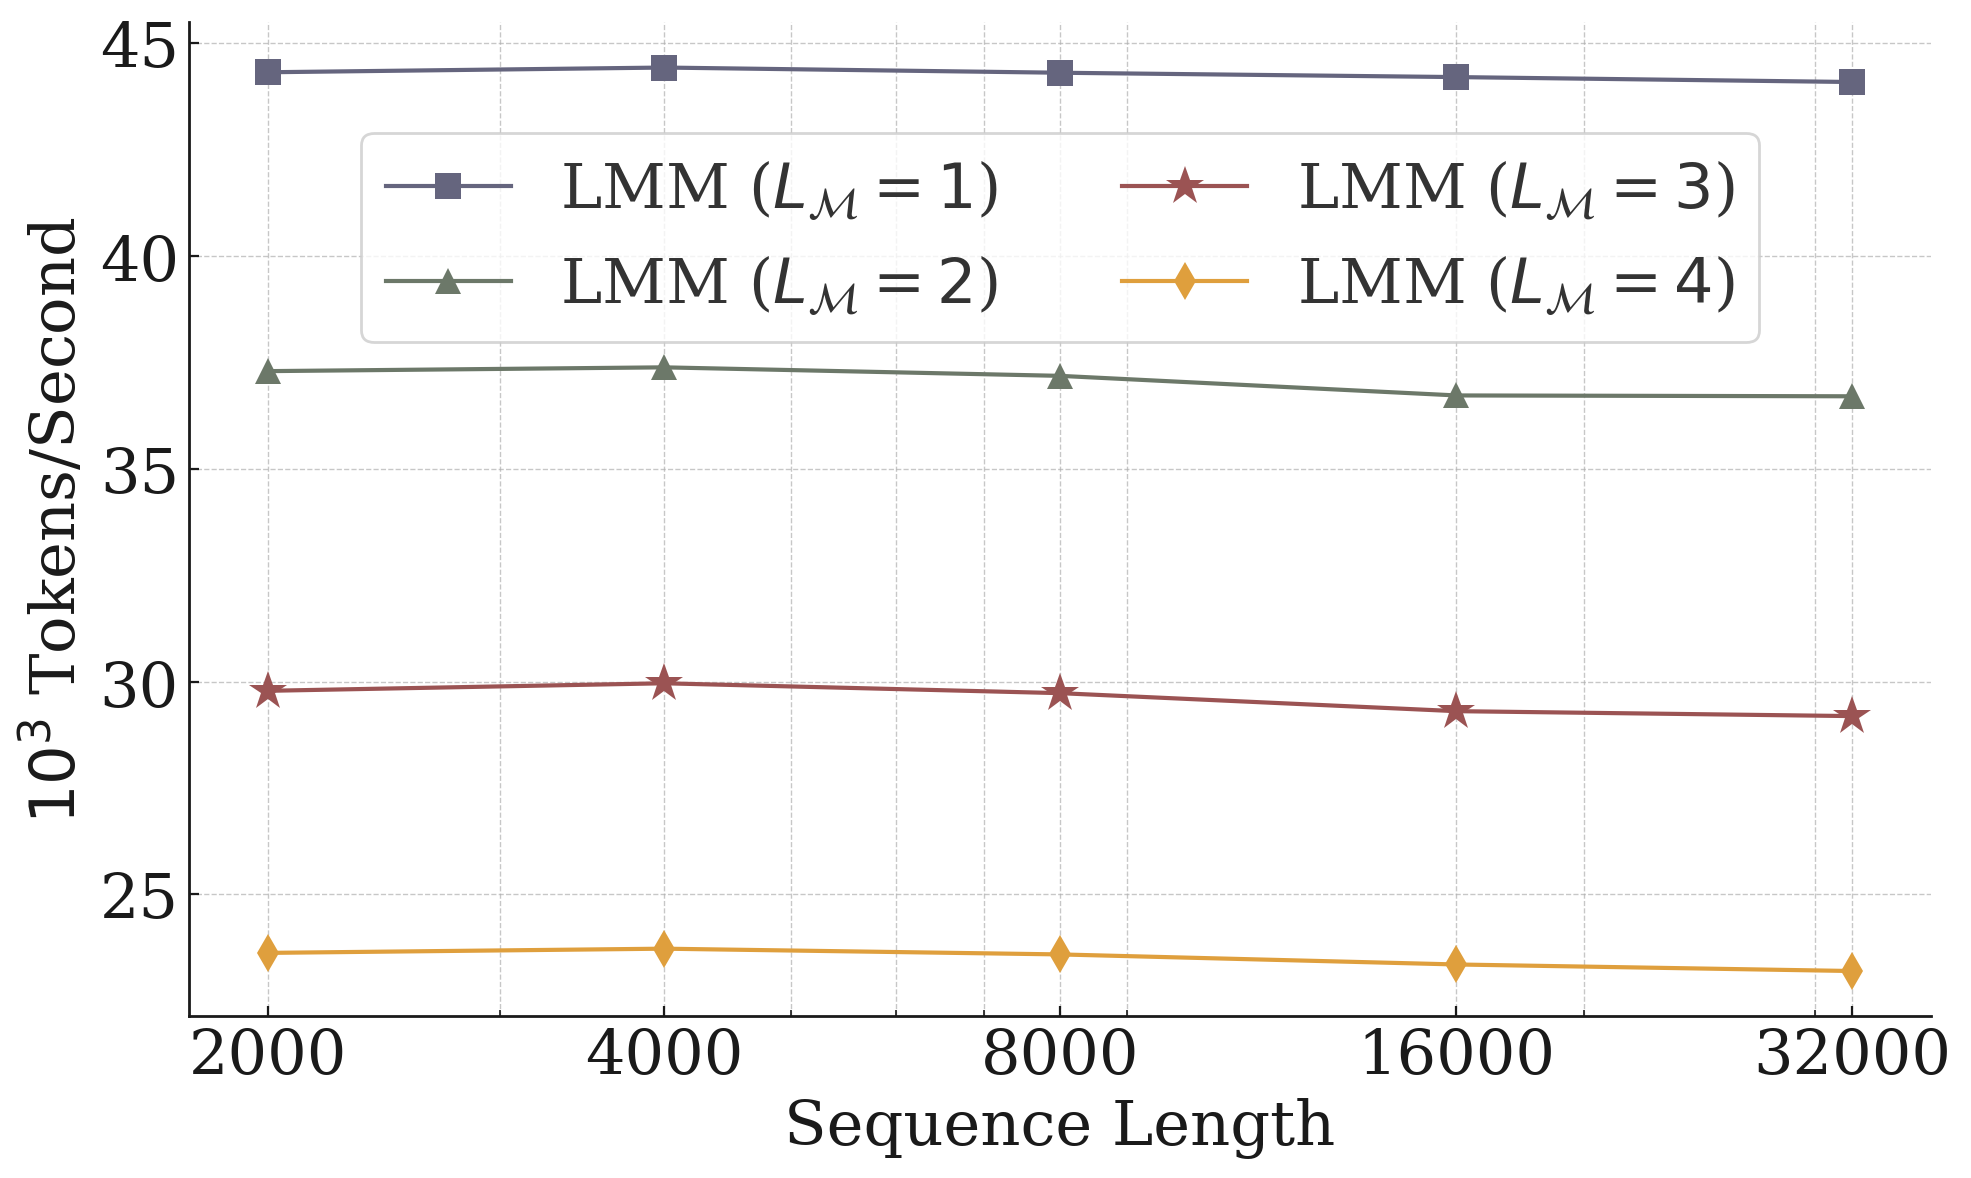
\includegraphics[width=\linewidth]{Figures/deep-memory-efficiency.png}
    \caption{The effect of memory depth on training throughput}
    \label{fig:effect-deep-memory-efficiency}
    \vspace{-8ex}
\end{wrapfigure}

We also evaluate the effect of memory depth ($L_{\M} = 1, 2, 3, 4$) on the training throughput. We report the training throughput (the number of tokens per second) as the function of sequence length in \autoref{fig:effect-deep-memory-efficiency}. All models scale linearly with respect to the context length (i.e., constant trend in the number of tokens per second with respect to sequence length). Also, by increasing the memory depth, as expected, we can see a linear trend that a deeper memory results in a slower training. Therefore, it is not always efficient to use deeper memory modules, showing a trade-off between effectiveness and efficiency. 


\begin{table*}[t!]
\centering
  \caption{\small Performance on long-term forecasting. The best results are \hspace{-1pt} \colorbox{myblue}{highlighted}\hspace{-1pt}. }\label{tab:avg_baseline_results}
  \centering
  \resizebox{0.9\linewidth}{!}{
  \centering
  \begin{tabular}{l| cc|  cc|  cc| cc| cc| cc| cc| cc| cc}
    \toprule
    \multicolumn{1}{c}{\multirow{2}{*}{}} & 
    \multicolumn{2}{c}{\rotatebox{0}{\scalebox{0.8}{\textbf{Neural Memory}}}} &
    \multicolumn{2}{c}{\rotatebox{0}{\scalebox{0.8}{\textbf{Simba}}}}&
    \multicolumn{2}{c}{\rotatebox{0}{\scalebox{0.8}{\textbf{iTransformer}}}} &
    \multicolumn{2}{c}{\rotatebox{0}{\scalebox{0.8}{\textbf{RLinear}}}} &
    \multicolumn{2}{c}{\rotatebox{0}{\scalebox{0.8}{\textbf{PatchTST}}}} &
    \multicolumn{2}{c}{\rotatebox{0}{\scalebox{0.8}{\textbf{Crossformer}}}}  &
    \multicolumn{2}{c}{\rotatebox{0}{\scalebox{0.8}{\textbf{TiDE}}}} &
    \multicolumn{2}{c}{\rotatebox{0}{\scalebox{0.8}{{\textbf{TimesNet}}}}} &
    \multicolumn{2}{c}{\rotatebox{0}{\scalebox{0.8}{\textbf{DLinear}}}} \\
    \cmidrule(lr){2-3} \cmidrule(lr){4-5}\cmidrule(lr){6-7}\cmidrule(lr){8-9} \cmidrule(lr){10-11} \cmidrule(lr){12-13} \cmidrule(lr){14-15} \cmidrule(lr){16-17} \cmidrule(lr){18-19}  
    \multicolumn{1}{c}{}  &  \multicolumn{1}{c}{\scalebox{0.78}{MSE}} & \multicolumn{1}{c}{\scalebox{0.78}{MAE}} &  \multicolumn{1}{c}{\scalebox{0.78}{MSE}} & \multicolumn{1}{c}{\scalebox{0.78}{MAE}} & \multicolumn{1}{c}{\scalebox{0.78}{MSE}} & \multicolumn{1}{c}{\scalebox{0.78}{MAE}}  & \multicolumn{1}{c}{\scalebox{0.78}{MSE}} & \multicolumn{1}{c}{\scalebox{0.78}{MAE}}  & \multicolumn{1}{c}{\scalebox{0.78}{MSE}} & \multicolumn{1}{c}{\scalebox{0.78}{MAE}}  & \multicolumn{1}{c}{\scalebox{0.78}{MSE}} & \multicolumn{1}{c}{\scalebox{0.78}{MAE}}  & \multicolumn{1}{c}{\scalebox{0.78}{MSE}} & \multicolumn{1}{c}{\scalebox{0.78}{MAE}}  & \scalebox{0.78}{MSE} & \multicolumn{1}{c}{\scalebox{0.78}{MAE}} & \multicolumn{1}{c}{\scalebox{0.78}{MSE}} & \multicolumn{1}{c}{\scalebox{0.78}{MAE}}  \\
    \midrule
    \midrule
    
    \scalebox{0.95}{ETTm1} & \scalebox{0.78}{\cellcolor{myblue}{0.358}} &\scalebox{0.78}{\cellcolor{myblue}{0.387}} &  \scalebox{0.78}{0.383} &\scalebox{0.78}{0.396}  & \scalebox{0.78}{0.407} & \scalebox{0.78}{0.410} & \scalebox{0.78}{0.414} & \scalebox{0.78}{0.407} &  {\scalebox{0.78}{0.387}} &  {\scalebox{0.78}{0.400}} & \scalebox{0.78}{0.513} & \scalebox{0.78}{0.496} & \scalebox{0.78}{0.419} & \scalebox{0.78}{0.419} & {\scalebox{0.78}{0.400}} & {\scalebox{0.78}{0.406}}  &{\scalebox{0.78}{0.403}} &{\scalebox{0.78}{0.407}}  \\ %&\scalebox{0.78}{0.961} &\scalebox{0.78}{0.734} \\
    % \midrule
    
    \scalebox{0.95}{ETTm2} & \scalebox{0.78}{\cellcolor{myblue}{0.261}} &\scalebox{0.78}{\cellcolor{myblue}{0.309}} &  \scalebox{0.78}{0.271} &\scalebox{0.78}{0.327}  & {\scalebox{0.78}{0.288}} & {\scalebox{0.78}{0.332}} &  {\scalebox{0.78}{0.286}} &  {\scalebox{0.78}{0.327}} &  {\scalebox{0.78}{0.281}} &  {\scalebox{0.78}{0.326}} & \scalebox{0.78}{0.757} & \scalebox{0.78}{0.610} & \scalebox{0.78}{0.358} & \scalebox{0.78}{0.404} &{\scalebox{0.78}{0.291}} &{\scalebox{0.78}{0.333}} &\scalebox{0.78}{0.350} &\scalebox{0.78}{0.401}   \\ %&\scalebox{0.78}{1.410} &\scalebox{0.78}{0.810} \\
    % \midrule
    
    \scalebox{0.95}{ETTh1} & \scalebox{0.78}{\cellcolor{myblue}{0.420}} &\scalebox{0.78}{\cellcolor{myblue}{0.421}} &  \scalebox{0.78}{0.441} &\scalebox{0.78}{0.432} & {\scalebox{0.78}{0.454}} &  {\scalebox{0.78}{0.447}} &  {\scalebox{0.78}{0.446}} &  {\scalebox{0.78}{0.434}} & \scalebox{0.78}{0.469} & \scalebox{0.78}{0.454} & \scalebox{0.78}{0.529} & \scalebox{0.78}{0.522} & \scalebox{0.78}{0.541} & \scalebox{0.78}{0.507} &\scalebox{0.78}{0.458} &{\scalebox{0.78}{0.450}} &{\scalebox{0.78}{0.456}} &{\scalebox{0.78}{0.452}}  \\ %&\scalebox{0.78}{1.040} &\scalebox{0.78}{0.795} \\
    % \midrule

    \scalebox{0.95}{ETTh2} & \scalebox{0.78}{\cellcolor{myblue}{0.336}} &\scalebox{0.78}{\cellcolor{myblue}{0.382}} &  \scalebox{0.78}{0.361} &\scalebox{0.78}{0.391}  &  {\scalebox{0.78}{0.383}} &  {\scalebox{0.78}{0.407}} &  {\scalebox{0.78}{0.374}} &  {\scalebox{0.78}{0.398}} & {\scalebox{0.78}{0.387}} & {\scalebox{0.78}{0.407}} & \scalebox{0.78}{0.942} & \scalebox{0.78}{0.684} & \scalebox{0.78}{0.611} & \scalebox{0.78}{0.550}  &{\scalebox{0.78}{0.414}} &{\scalebox{0.78}{0.427}} &\scalebox{0.78}{0.559} &\scalebox{0.78}{0.515}  \\ %&\scalebox{0.78}{4.431} &\scalebox{0.78}{1.729} \\
    % \midrule
    
    \scalebox{0.95}{ECL} & \scalebox{0.78}{\cellcolor{myblue}{0.162}} &\scalebox{0.78}{\cellcolor{myblue}{0.261}} &\scalebox{0.78}{0.169} &\scalebox{0.78}{0.274} &  {\scalebox{0.78}{0.178}} &  {\scalebox{0.78}{0.270}} & \scalebox{0.78}{0.219} & \scalebox{0.78}{0.298} & \scalebox{0.78}{0.205} &  {\scalebox{0.78}{0.290}} & \scalebox{0.78}{0.244} & \scalebox{0.78}{0.334} & \scalebox{0.78}{0.251} & \scalebox{0.78}{0.344} & {\scalebox{0.78}{0.192}} &\scalebox{0.78}{0.295} &\scalebox{0.78}{0.212} &\scalebox{0.78}{0.300}  \\ %&\scalebox{0.78}{0.311} &\scalebox{0.78}{0.397} \\
    % \midrule


    % \midrule
    
    \scalebox{0.95}{Traffic} & \scalebox{0.78}{\cellcolor{myblue}{0.415}} &\scalebox{0.78}{{0.289}} &  \scalebox{0.78}{0.493} &\scalebox{0.78}{0.291} &  {\scalebox{0.78}{0.428}} &  {\cellcolor{myblue}\scalebox{0.78}{0.282}} & \scalebox{0.78}{0.626} & \scalebox{0.78}{0.378} &  {\scalebox{0.78}{0.481}} &  {\scalebox{0.78}{0.304}}& \scalebox{0.78}{0.550} &  {\scalebox{0.78}{0.304}} & \scalebox{0.78}{0.760} & \scalebox{0.78}{0.473} &{\scalebox{0.78}{0.620}} &{\scalebox{0.78}{0.336}} &\scalebox{0.78}{0.625} &\scalebox{0.78}{0.383}   \\ %&\scalebox{0.78}{0.764} &\scalebox{0.78}{0.416} \\
    % \midrule
    
    \scalebox{0.95}{Weather} & \scalebox{0.78}{\cellcolor{myblue}{0.231}} &\scalebox{0.78}{\cellcolor{myblue}{0.265}} &  \scalebox{0.78}{0.255} &\scalebox{0.78}{0.280} &  {\scalebox{0.78}{0.258}} &  {\scalebox{0.78}{0.278}} & \scalebox{0.78}{0.272} & \scalebox{0.78}{0.291} &  {\scalebox{0.78}{0.259}} &  {\scalebox{0.78}{0.281}} & \scalebox{0.78}{0.259} & \scalebox{0.78}{0.315} & \scalebox{0.78}{0.271} & \scalebox{0.78}{0.320} &{\scalebox{0.78}{0.259}} &{\scalebox{0.78}{0.287}} &\scalebox{0.78}{0.265} &\scalebox{0.78}{0.317} \\ %&\scalebox{0.78}{0.634} &\scalebox{0.78}{0.548} \\
    \bottomrule
  \end{tabular}
  }
% \vspace{-4ex}
\end{table*}

\vspace{2ex}
\subsection{Time Series Forecasting}\label{sec:exp-timeseries}
To show the effectiveness of our memory module in a broader tasks, we also evaluate its performance in time series forecasting tasks. To this end, we use Simba framework~\citep{patro2024simba} for time series forecasting, and replace its Mamba module with our neural memory. We report the results on common time series forecasting benchmark datasets–ETT, ECL, Traffic, and Weather~\citep{zhou2021informer}. The results are reported in \autoref{tab:avg_baseline_results}. Our neural memory module is outperforming all baselines, including Mamba-based, linear-based, and Transformer-based architectures. 




\begin{table*}[t!]
\centering
\caption{Downstream evaluation of pre-trained DNA models on GenomicsBenchmarks~\citep{grevsova2023genomic}. We report top-1 classification accuracy ($\%$).}
\label{table:genomics_benchmarks}
\resizebox{0.75\linewidth}{!}{
\begin{tabular}{@{}lccccc@{}}
\toprule
Model       & Enhancer Cohn & Enhancer Ens & Human Reg. & Non-TATA Promoters & Human OCR Ens. \\ \midrule
CNN           & 69.5                 & 68.9                     & 93.3             & 84.6                     & 68.0               \\
DNABERT       & 74.0                 & 85.7                     & 88.1             & 85.6                     & 75.1               \\
GPT           & 70.5                 & 83.5                     & 91.5             & 87.7                     & 73.0               \\
HyenaDNA      & 74.2                 & 89.2                     & \cellcolor{myblue}93.8    & 96.6                     & \cellcolor{myblue}80.9      \\ \midrule
Transformer++ & 73.4                 & {89.5}            & 89.9             & 94.4                     & 79.5               \\
Mamba         & 73.0                 & -                        & -                & 96.6                     & -                  \\
Based         & {74.6}        & 89.5            & 89.5             & \cellcolor{myblue}96.8            & 79.0               \\ 
\midrule
Neural Memory Module & \cellcolor{myblue}75.2 &  \cellcolor{myblue}89.6 & 89.3 & 96.6 & 79.9\\
% Titans (MAG) & & & & & \\
% Titans (MAL) & & & & & \\
\bottomrule
\end{tabular}
}
\end{table*}

\subsection{DNA Modeling}\label{sec:exp-DNA}
In order to understand the capability of Titans beyond natural language, we further evaluate the performance of our neural memory module on DNA modeling tasks. To this end, we evaluate pre-trained models on the downstream tasks in GenomicsBenchmarks~\citep{grevsova2023genomic}. We follow the same experimental setups from \citet{nguyen2024hyenadna}, and re-use the reported results of baselines by \citet{arora2024simple}. The performance of Titans (LMM) and baselines are reported in \autoref{table:genomics_benchmarks}.  We find that LMM is competitive with state-of-the-art architectures across different downstream genomics tasks.





\subsection{Efficiency}\label{sec:exp-efficiency}
\begin{wrapfigure}{r}{0.33\linewidth}
    \centering
    \vspace{-3ex}
        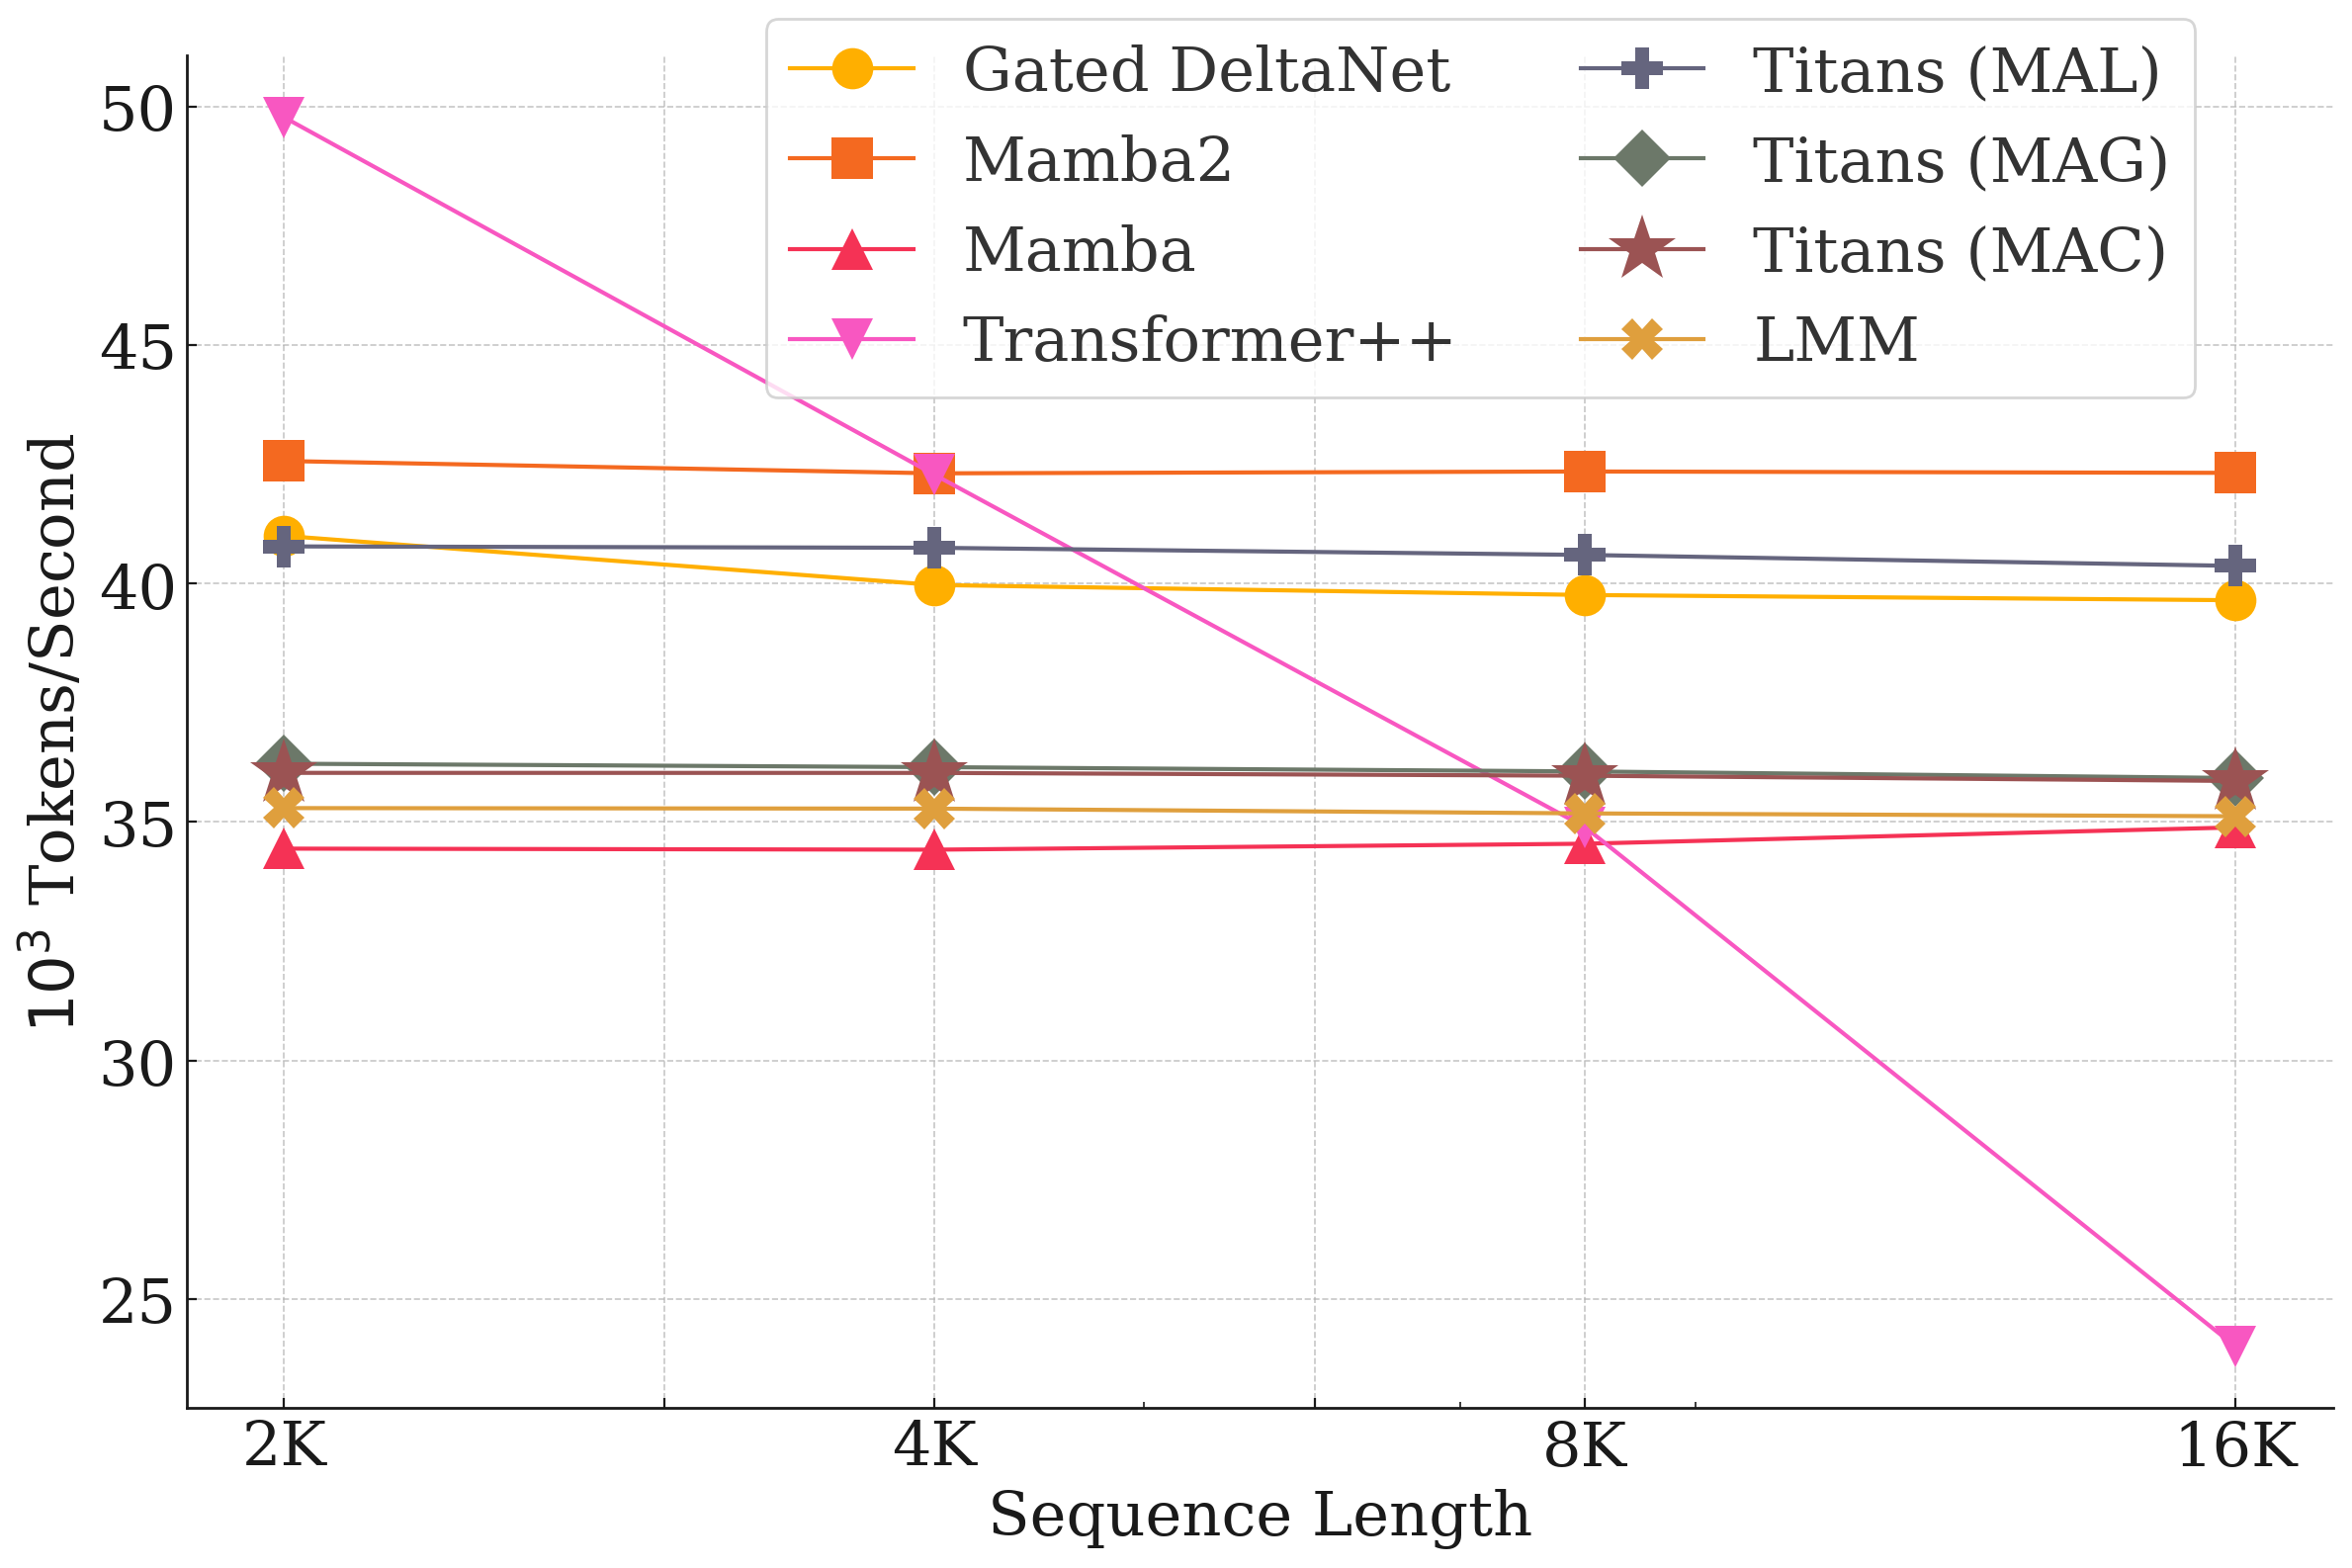
\includegraphics[width=\linewidth]{Figures/efficiency.png}
    \caption{Training throughput comparison of Titans and baselines. }
    \label{fig:efficiency}
    \vspace{-6ex}
\end{wrapfigure}
In this part, we compare the efficiency of our neural memory as well as Titans with state-of-the-art sequence models. The training throughput of models for different \texttt{sequence length $\times$ batch size} are reported in \autoref{fig:efficiency}. Comparing recurrent models, including our neural memory module, we can see our memory module is slightly slower than Mamba2 and Gated DeltaNet, mainly due to: (1) having deep memory and more expressive
transition process (memory update), and (2) highly optimized kernel in the implementation of Mamba2. Interestingly, Titans (MAL) are faster than baselines as well as the memory module. The main reason for this better throughput is the highly optimized kernel of Flash-Attention~\citep{dao2024flashattention}, which is used for implementing SWA and full attention module in Titans.  



\subsection{Ablation Study}\label{sec:exp-ablation}
Finally, we perform ablation studies on the different architectural choices in Titans. We consider our neural memory module as a base model and then changing one component at a time: (1) replacing deep memory with linear memory, removing (2) convolution, (3) momentum in the surprise measure, (4) weight decay (or forgot mechanism), and (5) persistent memory. The results are reported in \autoref{tab:ablation}. All components of neural memory design are positively contributing to its performance, where the greatest contribution comes from weight decay, momentum, convolution, and persistent memory, respectively. 




\begin{table*}
    \centering
    \caption{Ablation Study on Titans. All components of Titans are positively contributing to its performance. }
    \label{tab:ablation}
    \resizebox{0.55\linewidth}{!}{
    \begin{tabular}{l c c c}
    \toprule
    \multirow{2}{*}{Model}     & Language Modeling & Reasoning & Long Context\\
    & ppl $\downarrow$ & acc $\uparrow$ & acc $\uparrow$ \\
    \midrule
    \midrule
    LMM         &   \cellcolor{mygreen}27.01  &   \cellcolor{mygreen}47.83  & \cellcolor{mygreen}92.68\\ 
    \midrule
    \hspace{6pt}+\texttt{Attn} (MAC) & 26.67 & \cellcolor{myblue}48.65 &       \cellcolor{myblue}{97.95}         \\
    \hspace{6pt}+\texttt{Attn} (MAG) & \cellcolor{myblue}25.70 & 48.60 & 96.70               \\
    \hspace{6pt}+\texttt{Attn} (MAL) & 25.91 & 47.87 &  96.91              \\
    \midrule
    Linear Memory          &  28.49   &  46.97   &  85.34 \\
    w/o Convolution        &  28.73   &  45.82   &  90.28\\
    w/o Momentum           &  28.98   &  45.49   &  87.12\\
    w/o Weight Decay       &  29.04   &  45.11   &  85.60\\
    w/o Persistent Memory  &  27.63   &  46.35   &  92.49\\
    \toprule
    \end{tabular}
    }
\end{table*}

\head{The Effect of Architectural Design}
To evaluate the effect of architecture design, we compare the performance of three represented variants of Titans in three aspects of (i) language modeling, (ii) commen-sense reasoning, and (iii) long context NIAH (BABILong) tasks. The results are reported in \autoref{tab:ablation}. We find that MAC and MAG have close performance in language modeling and common-sense reasoning tasks, while MAC achieve significantly better performance in long-context NIAH. Both of these models achieve better performance than MAL. These results along with \autoref{fig:efficiency}, show a trade-off between fast training and more expressive design.  